% Using template for a Computer Science Tripos Part II project dissertation
\documentclass[12pt,a4paper,twoside,openright]{report}
\usepackage[pdfborder={0 0 0}]{hyperref}    % turns references into hyperlinks
\usepackage[margin=25mm]{geometry}  % adjusts page layout
\usepackage{graphicx}  % allows inclusion of PDF, PNG and JPG images
\usepackage{verbatim}
\usepackage{docmute}   % only needed to allow inclusion of proposal.tex
\usepackage{natbib}
\usepackage{tikz}
\usepackage{wasysym}
\usepackage{amssymb}
\usepackage{textcomp}

\raggedbottom                           % try to avoid widows and orphans
\sloppy
\frenchspacing
\clubpenalty1000%
\widowpenalty1000%
\parindent 0pt
\parskip 6pt

\renewcommand{\baselinestretch}{1.1}    % adjust line spacing to make
                                        % more readable

\begin{document}

%%%%%%%%%%%%%%%%%%%%%%%%%%%%%%%%%%%%%%%%%%%%%%%%%%%%%%%%%%%%%%%%%%%%%%%%
% Title


\pagestyle{empty}

\rightline{\LARGE \textbf{Z\'ebulon Goriely}}

\vspace*{60mm}
\begin{center}
\Huge
\textbf{Simulating Language Learning and Evolution} \\[5mm]
Computer Science Tripos -- Part II \\[5mm]
Queens' College \\[5mm]
\today  % today's date
\end{center}

%%%%%%%%%%%%%%%%%%%%%%%%%%%%%%%%%%%%%%%%%%%%%%%%%%%%%%%%%%%%%%%%%%%%%%%%%%%%%%
% Proforma, table of contents and list of figures

\pagestyle{plain}

\chapter*{Proforma}

{\large
\begin{tabular}{ll}
Name:               & \bf Z\'ebulon Goriely                       \\
College:            & \bf Queens' College                     \\
Project Title:      & \bf Simulating Language Learning and Evolution \\
Examination:        & \bf Computer Science Tripos -- Part II, May 2020  \\
Word Count:         & \bf NULL\footnotemark[1]  \\
Project Originator: & Z\'ebulon Goriely                    \\
Supervisor:         & Prof. Paula Buttery and Dr. Andrew Caines                  \\ 
\end{tabular}
}
\footnotetext[1]{This word count was computed
by \texttt{detex diss.tex | tr -cd '0-9A-Za-z $\tt\backslash$n' | wc -w}
}
\stepcounter{footnote}


\section*{Original Aims of the Project}

Language has evolved and therefore probably gave an evolutionary advantage to the individuals that exhibited it. According to \citet{Cangelosi1998}, it is difficult to investigate the evolutionary origin of language and the selective pressures that may have originated language due to the limited evidence available. They propose using computer simulations of evolutionary scenarios to investigate this. In the paper referenced, they describe a simulated toy world where agents controlled by neural networks interact with an environment of mushrooms that are edible and poisonous. Exploring this simulation is the basis of my project.

\section*{Work Completed}

I implemented the mushroom-world simulation and explored three populations of feed-forward neural networks; one without language, one with an externally imposed language and one with an evolved language. To simulate evolution, I implemented a genetic algorithm to allow the fittest members of each generation to reproduce. The state of the simulation was saved at each generation in order plot the fitness of the three populations, plot the quality of the language produced and investigate behavioural tests. To conclude the project, I compared these findings with \citet{Cangelosi1998}.

\section*{Special Difficulties}

None.
 
\newpage
\section*{Declaration}

I, Z\'ebulon Goriely of Queens' College, being a candidate for Part II of the Computer
Science Tripos, hereby declare
that this dissertation and the work described in it are my own work,
unaided except as may be specified below, and that the dissertation
does not contain material that has already been used to any substantial
extent for a comparable purpose.

\bigskip
\leftline{Signed Z\'ebulon Goriely}

\medskip
\leftline{Date [date]}

\tableofcontents

\listoffigures

\newpage
\section*{Acknowledgements}

Paula et al.

%%%%%%%%%%%%%%%%%%%%%%%%%%%%%%%%%%%%%%%%%%%%%%%%%%%%%%%%%%%%%%%%%%%%%%%
% Introduction

\pagestyle{headings}

\chapter{Introduction}

\emph{Introduction here, start again as if abstract does not exist. Include your contributions in bullet point format. End with paragraph describing structure of the rest of the paper}

\section{Motivations}

\emph{High level, still cite, why does this interest us from a scientific perspective. What could we learn.}

- Want to investigate evolutionary origin of language

- Difficult to investigate due to limited evidence, so computer simulations could be good

- Investigation of cultural vs sexual mechanisms

- Artificial life

- Main question - how can language evolve when it has a purely informative function and so advantageous to receiver but not to the producer?

- Reference Clark (1993) for what an efficient language is

\section{Prior Work}

\emph{State what similar work has been done before and since what i'm trying to replicate. Also a continuation of the motivation. Why does this paper in particular interest you. Focus more on their prior work. Talk about work that has continued.}

- Symbol grounding

- Language games

- Mushroom world

\section{Project Overview}

%%%%%%%%%%%%%%%%%%%%%%%%%%%%%%%%%%%%%%%%%%%%%%%%%%%%%%%%%%%%%%%%%%%%%%%%%%%%
% Preparation

\chapter{Preparation}\label{chapter:preparation}

\emph{This chapter covers the background to my project in Sections \ref{section:world} to \ref{section:analysis}, then evaluates the requirements for the project in Section \ref{section:requirements}. I discuss the starting point of my project in Section \ref{section:starting} and the software engineering techniques used in Section \ref{section:software}.}

\section{Mushroom World}\label{section:world}

To explore how the introduction of language may affect a population's fitness, we need a simulated environment in which to test these changes. This ``mushroom world'' was described by \cite{Cangelosi1998}, inspired by the use of signals to communicate information about food location and quality present in may species.

The organisms will live in an environment populated by two different types of mushroom; edible and poisonous. The organisms will reproduce based on their ability to eat edible mushrooms and avoid the poisonous ones. They will need to learn to categorise the two mushrooms and respond accordingly by moving towards and eating the edible mushrooms and moving away from the poisonous mushrooms.

To ensure this categorisation isn't trivial for the organisms, the mushrooms will have different properties. Edible mushrooms will resemble each other but won't be identical and likewise for poisonous mushrooms.

Each organism will live in an environment of $20 \times 20$ cells containing 20 randomly distributed mushrooms; 10 of which are poisonous and 10 of which are poisonous. They will be able to explore this world in 15 epochs of 50 simulation cycles each; in each new epoch the world is 'reset', the position of the entity reset in a new environment with 20 new randomly distributed mushrooms. An example of this world can be seen in Figure \ref{fig:environment}.

\begin{figure}[h]
\centering
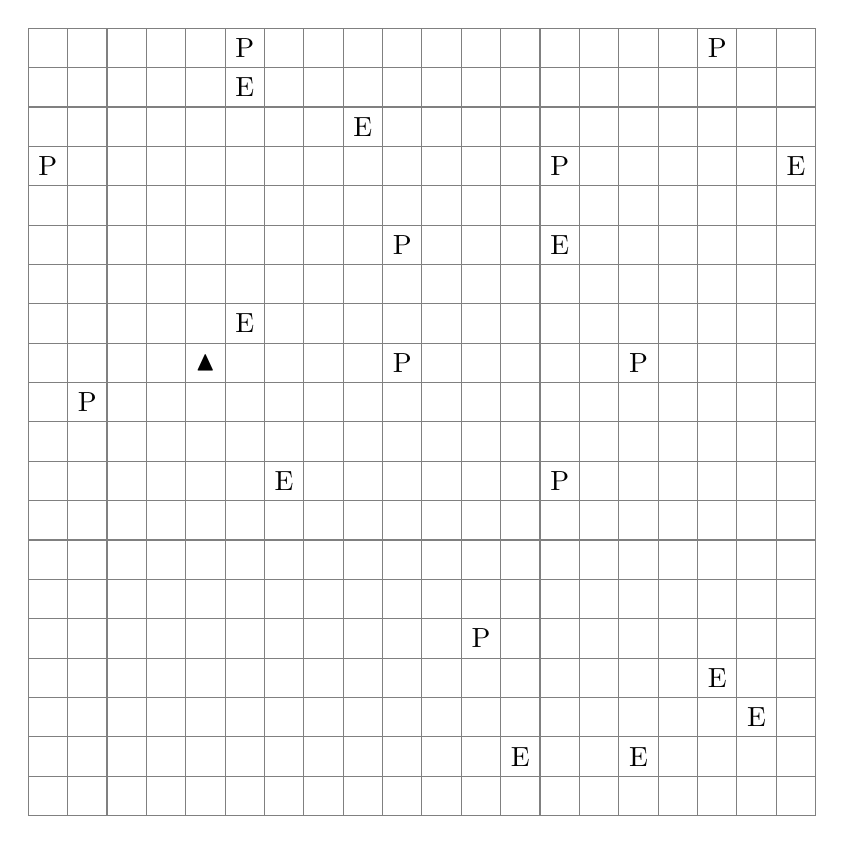
\begin{tikzpicture}
\draw[step=0.5cm,color=gray] (0,0) grid (10,10);
\node at (6.75,8.25){P};
\node at (5.75,2.25){P};
\node at (4.75,5.75){P};
\node at (6.75,4.25){P};
\node at (8.75,9.75){P};
\node at (4.75,7.25){P};
\node at (2.75,9.75){P};
\node at (0.25,8.25){P};
\node at (0.75,5.25){P};
\node at (7.75,5.75){P};
\node at (9.75,8.25){E};
\node at (2.75,9.25){E};
\node at (9.25,1.25){E};
\node at (8.75,1.75){E};
\node at (3.25,4.25){E};
\node at (2.75,6.25){E};
\node at (4.25,8.75){E};
\node at (6.75,7.25){E};
\node at (7.75,0.75){E};
\node at (6.25,0.75){E};
\node at (2.25,5.75){$\blacktriangle$};
\end{tikzpicture}
\caption{An organism ($\blacktriangle$) in the simulation environment with edible (E) and poisonous (P) mushrooms.}
\label{fig:environment}
\end{figure}

These constants are fairly arbitrarily chosen by Cangelosi and in later sections I will explore the effects of changing them, but for now I can intuitively explain some of these choices. The 15 epochs are used to average out the randomly generated positions of mushrooms so that it is really the behaviour of the organism that is being tested, not the random choice of environment. The 50 simulation cycles along with the specific dimensions of the environment ensures that the organism will likely be able to reach at least one edible mushroom but will unlikely be able to eat all edible mushrooms in time. This encourages productive strategies to search for edible mushrooms within the limited time available. Intuitively, this reflects the limited time that living organisms have to search for food in their lifetimes. A full list of constants can be seen in Table \ref{table:constants}.

\section{Entities}\label{section:entities}

In the simulation, organisms are represented by \emph{entities}. Entities can \emph{perceive} their surroundings and \emph{act} accordingly.

The perception is composed of three senses; the entity can sense the \emph{direction} of the nearest mushroom (a sort of `smelling' sense), can see the \emph{properties} of mushrooms it is adjacent to (a `visual' sense) and can receive \emph{signals} from other entities (a 'auditory' sense). The adjacency restriction to the visual sense means that entities without any other signals must approach mushrooms in order to be able to categorise them.

The action is composed of two responses; the \emph{movement} of the entity and the \emph{signal} it produces. The movement is restricted to four options; moving one cell forwards, turning 90\textdegree~left, turning 90\textdegree~right and doing nothing. Instead of incorporating some `eat' action, a mushroom will be considered eaten when the entity moves into the cell that the mushroom occupies. The signal is used to communicate information to other entities when we explore adding language to the simulation.

The simulation should also incorporate evolution; some process by which the fittest entities of a species reproduce to pass on their behaviour to a new generation, with some degree of mutation. This will allow a population's average fitness to improve over many generations. From this abstract description of entities, I can consider how this system may be designed.

\subsection{Feed-Forward Neural Networks}\label{section:neural}

Inspired by the biological neural networks that constitute animal brains, \emph{artificial neural networks} are an appropriate choice for modelling the behaviour of these entities. Neural networks are composed of nodes (artificial neurons) which loosely model the neurons in a biological brain. Each node processes a signal by computing a non-linear function of the sum of the inputs. By organising these nodes into layers, signals can travel through from the input layer to the output layer. This is a \emph{feed-forward} neural network as there are no loops present to allow a signal to traverse a layer multiple times. A \emph{fully-connected} neural network feeds the output of every node in a layer into the input of every node in the next layer. 

Each node computes an input using a \emph{propagation function} as a weighted sum of the outputs of predecessor nodes, incorporating a \emph{bias} added to the result of the propagation. An \emph{activation function} can then be applied to produce the output of the node. As Cangelosi does not describe which activation function was used in his paper, I will explore the use of three common functions:

\begin{itemize}
	\item Identity: $f(x) = x$
	\item Sigmoid: $f(x) = \frac{1}{1+e^{-x}}$
	\item ReLU\footnote{ReLU stands for Rectified Linear Unit}:	$ f(x) = 
    \left\{
        \begin{array}{ll}
          0~\mathrm{for}~x \leq 0 \\
          x~\mathrm{for}~x > 0
        \end{array}
      \right.
      $
\end{itemize}

The entities can be represented by a fully-connected feed-forward neural network. The  \emph{perception} of the entity acts as the input of the neural network with the output treated as the \emph{action} chosen by the entity. To increase the computational abilities of the entity, I also include a layer of hidden nodes to allow for more complex decision making (INCLUDE REASON WHY HERE). This structure can be seen in Figure \ref{fig:neuralnet}. By altering the weights and biases used by the network, the entity will respond differently to the perceptual inputs, producing different behaviours. 

\begin{figure}[t]
  \centering
  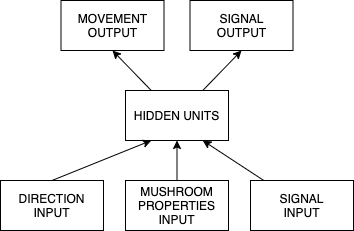
\includegraphics[width=.6\linewidth]{figs/NeuralNets}
  \caption{Structure of a fully-connected ANN to control entity behaviour}
  \label{fig:neuralnet}
\end{figure}

\subsection{Alternative Structures}

- talk about linear regression

- talk about svms

- talk about more complex neural networks

\subsection{Genetic Algorithm}\label{section:genetic}

Similarly to how an artificial neural network is a natural implementation for simulating the behaviour of an entity, the \emph{genetic algorithm} is a natural implementation for simulating the population dynamics of a population of such entities. Just as artificial neural networks are inspired by animal brains, the genetic algorithm is inspired by the process of natural selection which is the very process that we want to simulate. 

Generally, a genetic algorithm takes a \emph{population} of candidate solutions to an optimisation problem and evolves the population towards a better solution. Each candidate has a set of properties, a \emph{genetic representation} which can be mutated and altered. The evolution starts from a population of randomly generated individuals and proceeds iteratively. For each \emph{generation}, the \emph{fitness} of each individual is calculated. The more fit individuals are selected and their genomes modified to form a new generation, used in the next iteration.

This maps neatly to our problem. The \emph{population} used by the algorithm is simply a group of entities. The \emph{genetic representation} of the entities is the set of weights and biases used by each neural network. The \emph{fitness} score, $F$ will be calculated according to the number of edible and poisonous mushrooms eaten by the entity during the simulation, $E$ and $P$ respectively:

\begin{equation}
\label{equation:fitness}
\mathrm{F} = 10 E- 11 P
\end{equation}

This rewards entities that eat edible mushrooms and punishes those that eat poisonous mushrooms. The difference in weight between these two scores gives a greater reward to the entities that eat more edible mushrooms than poisonous mushrooms as it punishes the greedy strategy of simply eating as many mushrooms as possible.

Finally, the reproduction occurs by selecting a percentage of the population with the highest fitness score and producing a small set of offspring for each of these individuals by randomly altering a percentage of the weights and biases in the neural network. In \cite{Cangelosi1998}, the top $20\%$ of entities are selected from a population of 100. Each of these entities produces five entities by randomly mutating $10\%$ of their weights and biases, producing a new generation of 100 entities. These introduce two new constants, as described in Table \ref{table:constants}.

\subsection{Population types}\label{section:populations}

To carry out the investigation of whether introducing language to a population increases its fitness, I will implement three different populations in the simulation. As described by \cite{Cangelosi1998}, these three populations differ in how the communication signals are used in the simulation environment. The three population types are:

\begin{itemize}
	\item No Language
	\item External Language
	\item Evolved Language
\end{itemize}

The population with no language acts as a baseline. The audio input to the neural network controlling the entity is set to a constant and the audio output is ignored. These entities cannot perceive the properties of the mushrooms unless they are adjacent; unlike the other populations they are not assisted by some linguistic signal.

The population with an externally provided language is slightly different. Here, I imagine that at the closest mushroom to the entity, another entity is present and can see the properties of the mushroom, generating an appropriate audio signal for the primary entity. The language is ``externally provided" because I will enforce that one signal is used for edible mushrooms and another is used for poisonous mushrooms without actually involving another entity in the simulation. 

The population with an evolved language is similar to the External Language population, but I will not enforce the use of particular signals. Instead, I will allow the population to derive its own signals. This will be done by pairing the primary entity with another randomly chosen entity at each simulation cycle. This second entity will be given same inputs as the primary entity as well as the properties of the closest mushroom, no matter the distance. This entity labels the mushroom for the primary entity. The audio output of this second entity will be used as the audio input to the primary entity; simulating a one-word utterance.

The differences between these populations can be seen in Figure \ref{fig:populations}.

\begin{figure}[t]
  \centering
  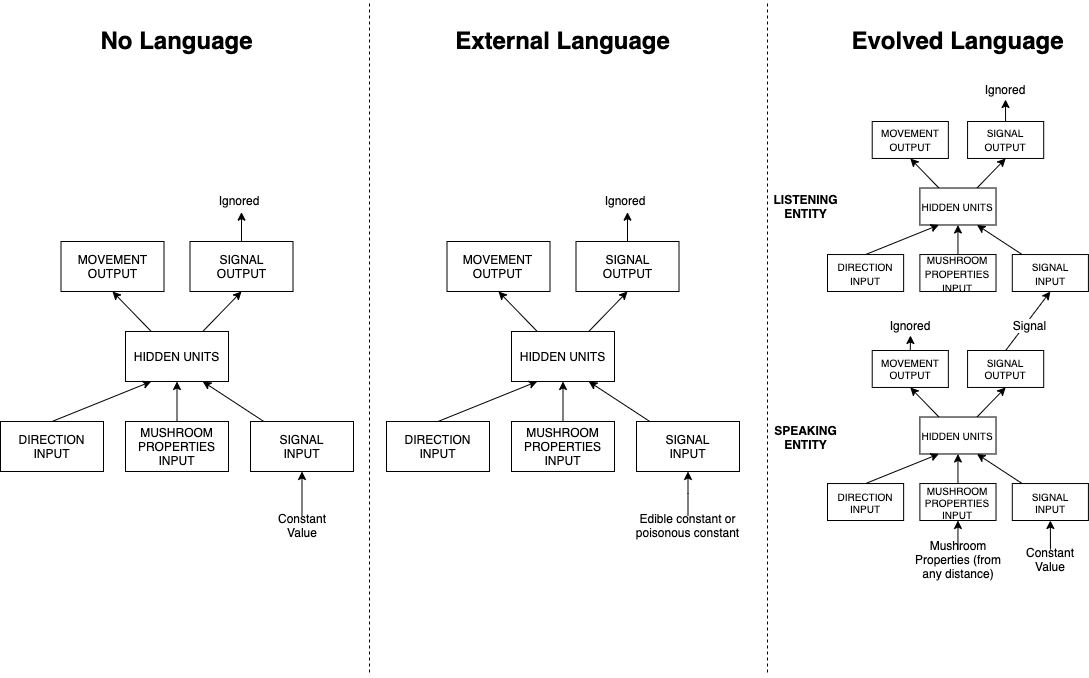
\includegraphics[width=.9\linewidth]{figs/populations}
  \caption{Differences in simulation structure for the three population types}
  \label{fig:populations}
\end{figure}

\begin{table*}[t]
\centering
 \begin{tabular}{ r | l | c}
 \bf{Constant} & \bf{Description} & \bf{Default Value} \\ [0.5ex] 
 \hline
dim\_x & The width of the simulation environment & 20 \\
dim\_y & The height of the simulation environment & 20 \\
num\_mushroom & The number of mushrooms placed in the environment & 20 \\
num\_epochs &  Number of epochs for each simulation & 15 \\ 
num\_cycles & Number of simulation cycles per epoch & 50 \\
num\_entities & Number of organisms in a population & 100 \\
num\_generations & Number of times a population will reproduce & 1000 \\
mutate\_percentage & The percentage of weights to mutate in reproduction & 10 \\
percentage\_keep & The percentage of organisms chosen to reproduce & 20 \\
\end{tabular}
\caption{A description of the constants and default values used for the simulation.}
\label{table:constants}
\end{table*}

\section{Simulation Analysis}\label{section:analysis}

\subsection{Generational Fitness}

As discussed in section \ref{section:genetic}, the fitness score for each entity describes its success in distinguishing between edible and poisonous mushrooms and correctly eating the former and avoiding the later. \cite{Cangelosi1998} plot the average fitness across 1000 generations to compare the three population types discussed in section \ref{section:populations}. This will be the primary way that I compare different runs of the simulation.

\subsection{Efficiency of Language}

\cite{Cangelosi1998} were also interested in the \emph{efficiency} of the language produced by these organisms. They gave three requirements for a population having an efficient language:

\begin{enumerate}
	\item Functionally distinct categories (e.g. mushroom type) are labelled with distinct signals
	\item A single signal tends to be used to label all instances within a category
	\item All the individuals in the population tend to use the same signal to label the same category
\end{enumerate}

These requirements were based on principles that \cite{Clark1995} argues govern a child's acquisition of a lexicon. To investigate the language produced by different populations, Cangelosi used a ``naming task''. In this controlled experiment, each entity in a population is exposed to the entire set of mushrooms (10 edible and 10 poisonous) in four locations (forward, left, backwards and right). This produces 80 signals per entity. The frequency distribution for the signals produced for edible and poisonous mushrooms by all entities can be plotted and this will be the second way I analyse the simulations.

\citet{Cangelosi1998} also described the calculation of a ``Quality Index'' (QI) to describe the efficiency of a language. The QI is calculated as follows:

$$d_{\mathrm{poisonous}} = \sum^{8}_{i = 1}{|x_i - x_e|}$$
$$d_{\mathrm{edible}} = \sum^{8}_{i = 1}{|y_i - y_e|}$$
$$\mathrm{QI} = \sum^{8}_{i = 1} |x_i - y_i| - k \times \min (d_{\mathrm{poisonous}}, d_{\mathrm{edible}})$$

$x_i$ and $y_i$ are the frequencies of signals used for poisonous and edible mushrooms respectively, as calculated from the ``naming task'' and $x_e$ and $y_e$ are the expected percentages in the case of a flat distribution. $k$ is a constant to weight the effect of the internal dispersion values $d_{\mathrm{poisonous}}$ and $d_{\mathrm{edible}}$ and is typically 1.

These dispersion values measure the variance of the distribution of signals used for the same category (edible or poisonous). This captures the use of synonyms, as these values are highest when only one signal is used for the category. 

The first part of the QI equation captures the principle of contrast (use of one word for each class of mushrooms) as it is highest when different signals are used for each category. By adding(?) this to the smaller of the two dispersion values, we get a score that captures the idea of an `efficient' language.

This will be the third way that I analyse the simulations; in particular I will examine the correlation between language efficiency and population fitness. In particular, it will be interesting to see if a correlation exists in the No Language population, despite not using any form of communication, as this would imply the parallel development of cognitive ability with linguistic ability.

LOOK INTO THIS EQUATION - A PLUS MAKES A LOT MORE SENSE

\section{Requirements Analysis}\label{section:requirements}

My project involves reimplementing the simulation described in sections \ref{section:world} - \ref{section:entities} and analysing this simulation in regards to the three metrics described in section \ref{section:analysis}. The requirements for this project can then be divided into two sections; implementing the simulation and constructing the means of analysis my implementation against the findings in \citet{Cangelosi1998}.

\subsection*{Implementing the Simulation}

\begin{enumerate}

\item Have a simulation environment with a world grid populated by poisonous and edible mushrooms as described in section \ref{section:world}. The simulation loop should be divided into regular `epochs'.

\item Have entities capable of navigating the environment, taking actions in each simulation cycle controlled by feedforward neural networks; with the structure described in section \ref{section:neural}.

\item Have a genetic algorithm that runs after all agents complete the simulation, as described in section \ref{section:genetic}.

\item Have three populations, one without language, one with an externally imposed language and one with an evolved language involving speaker-listening pairs, as described in section \ref{section:populations}.

\end{enumerate}

\subsection*{Analysis of the Simulation}

\begin{enumerate}

\item Have plots of the average fitness over the number of generations to compare between the three populations.

\item Have behavioural tests to investigate the behaviour of random individual organisms at specific generations.

\item Have plots the frequency distribution of the different signals produced by the individuals with the evolved language using a `naming task'.

\item Calculate the Quality Index (QI) of the language produced by the population without language and the population with an evolved language to investigate the genetic advantage of producing productive signals. 

\item Investigate the correlation between QI of the language and the fitness of the species to determine if change in the language or in the categorisation skill of the entities affects the linguistic ability.

\end{enumerate}

\section{Starting Point}\label{section:starting}

The implementation of the project is based on \citet{Cangelosi1998} which I familiarised myself with before beginning the project and in the early preporatory phases.

This project builds on concepts of simulations; I had a small amount of experience in programming simulations from an A-Level project in 2016. Before the project, I also read Simulating the Evolution of Language \citep{Cangelosi2002} to give me an overview of the techniques used in this field. 

This project builds on some of the content covered in the Artificial Intelligence course and the Formal Models of Language course form Part 1b. In particular, I had no experience with neural networks before beginning this project and all the code for the project was written from scratch and within the dates of the project.

\section{Software Engineering}\label{section:software}

\subsection{Languages and Libraries}

I chose Python for my project due to the ease of programming, my experience with it and the availability of good libraries for numerical analysis and plotting. To avoid code duplication, I made use of a few libraries:

\begin{enumerate}
 	\item To perform some scientific computing, I used SciPy\footnote{https://www.scipy.org/}.
	\item For the plotting of the analysis of the simulation, I used Matplotlib\footnote{https://matplotlib.org/}. 
	\item For producing unit tests, I used pytest\footnote{https://docs.pytest.org/}.
\end{enumerate}

\subsection{Project Management}

During implementation, I followed an agile development process. An initial project plan was formulated at the beginning of the project with a list of tasks to complete. These tasks were compiled into a Kanban board, with sections for Todo, In Progress, Testing/Documenting and Completed. My project plan divided the timeline of my project into a series of 2-3 week sprints, each with associated deadlines and milestones. At the beginning of each sprint I selected the tasks to complete in order to meet these deadlines and successfully pass each milestone, often completing additional tasks when work was completed early.

This agile process allowed me to ensure I was on track with my project. In fact, the success criteria proposed at the start of the project was met very early on in the timeline, allowing me to focus on refining the project and work on my extensions. 

\subsection{Version Control}

For version control, I used Git to track change with a remote repository on GitHub\footnote{https://github.com/}. This served as a backup, allowed me to revert to previous iterations of my code and allowed me to work on multiple computers. In particular, it allowed me to deploy my project to the University's High Performance Computing service for running the simulations, as discussed below. In addition, I also performed hardware backup to a hard drive twice a week.

\subsection{Development tools}

I made use of a number of tools to streamline my development process:

\begin{enumerate}
	\item I used Travis\footnote{https://travis-ci.org/} for continuous integration. With each commit, a script would automatically run all my unit tests and check my code for correct formatting.
	\item I used pylint\footnote{https://www.pylint.org/} to lint my code. This allowed me to ensure my code was readable and that I was complying with Google's python style guide\footnote{http://google.github.io/styleguide/pyguide.html}.
	\item I used yapf\footnote{https://github.com/google/yapf} to format my code consistently. I implemented a git hook to automatically format my code with each commit; the formatting was further checked by my Travis script.
\end{enumerate}

\subsection{Development environment}

I used Visual Studio Code\footnote{https://code.visualstudio.com/} as a development environment, due to the friendly interface and useful set of plugins that integrated nicely with git, pylint and pytest. 

To run my simulations, I used the University's High Performance Computing service. I created a set of Slurm scripts with a bash script that would allow me to schedule 30 simulations to run at once and independently. The results of these simulations were saved to files that I could copy to my local filesystem over SSH.

\subsection{Code License}

My source code is publicly available on GitHub with a README to explain how to use it. The project is licensed under the MIT license, for free modification and reuse while limiting my liability. It also preserves the copyright notice.

\section{Summary}\label{section:summary}

The evolution of language is an interesting problem that can be explored using simulations. In this project I will implement the ``mushroom world'' environment populated by entities controlled by neural networks with a genetic algorithm to model evolution. Three populations will be implemented; one without language, one with an external language and one with an evolved language. By comparing these populations in terms of fitness and language, I will be able to investigate the parallel development of the ability of the entities to categorise mushrooms and their ability to name them.

%%%%%%%%%%%%%%%%%%%%%%%%%%%%%%%%%%%%%%%%%%%%%%%%%%%%%%%%%%%%%%%%%%%%%%%
% Implementation

\chapter{Implementation}

\begin{figure}[t]
  \centering
  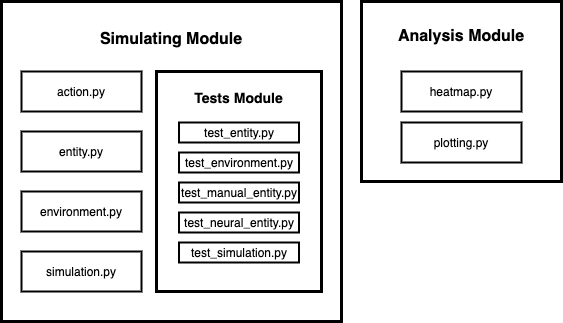
\includegraphics[width=.9\linewidth]{figs/modules}
  \caption{Core modules for my project}
  \label{fig:modules}
\end{figure}

\begin{figure}[t]
  \centering
  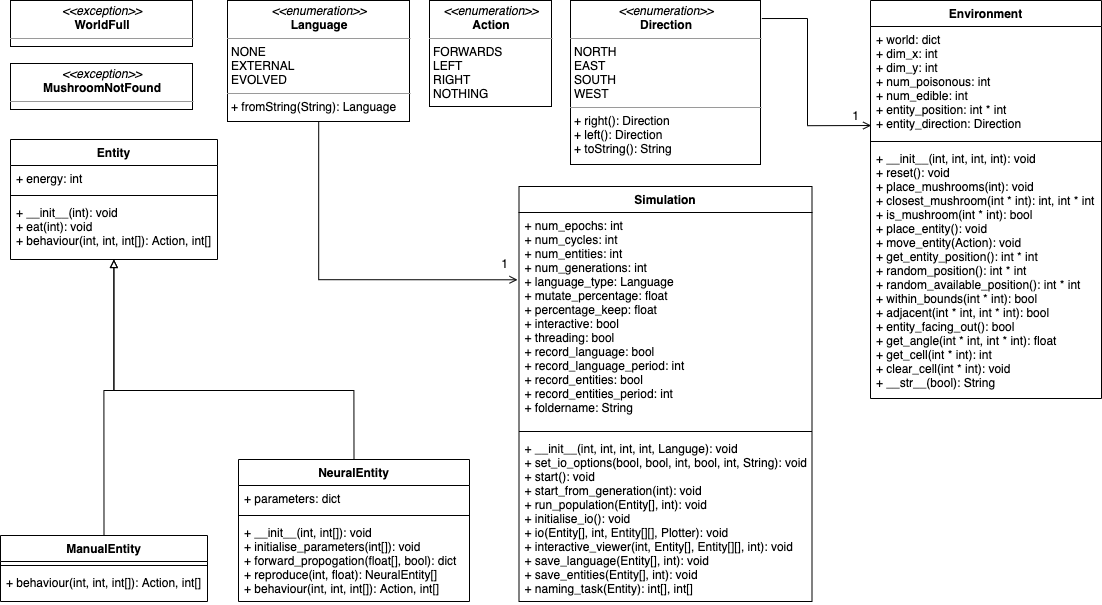
\includegraphics[width=.9\linewidth]{figs/uml}
  \caption{UML Diagram for the Simulating Module}
  \label{fig:uml}
\end{figure}

\emph{Talk about problems with trying to replicate, not knowing what you set.}

\section{High-level Overview}

The implementation of my project is split into three modules as seen in Figure \ref{fig:modules}. The Simulating module contains all the code relevant to creating the simulation. This covers the ``Implementing the Simulation'' requirements for the project described in section \ref{section:requirements}. The Analysis module contains functions for plotting different graphs and carrying out the ``Analysis of the Simulation'' requirements for the project. Finally, the Experiments module contains a series of functions used for quickly running different variants of the simulation. 

Within the Simulating module, the classes correspond to the core concepts detailed in Chapter 2. A full UML diagram of this module (excluding tests) can be seen in Figure \ref{fig:uml}. The Entity class and subclasses correspond to the entities described in \ref{section:entities}. The Environment class corresponds to the ``mushroom world'' simulation environment described in Section \ref{section:world}. The Simulation class corresponds to the actual simulation, including the genetic algorithm (\ref{section:genetic}) and the different populations (\ref{section:populations}).

The Analysis module contains the code to analyse the simulation. This includes the plotting of generational fitness, language frequency and quality index as described in \ref{section:analysis}.

\section{Environment}

The Environment modules contains the Direction enumeration and the Environment class. These are used to represent the state of the mushroom world including the position of the mushrooms and the entity and the direction that the entity is facing. It contains methods for populating the world with mushrooms, managing the state of the world and querying the world.

\subsection{Mushrooms}\label{section:mushrooms}

Mushrooms are represented as 10-bit integers. Conceptually, each bit corresponds to a binary property of the mushroom. Poisonous mushrooms are represented as the bit-string 0b1111100000 with one randomly-chosen bit flipped. Similarly, edible mushrooms are represented by the bit-string 0b0000011111, again with one bit flipped. This means that edible and poisonous mushrooms may share two or zero bits in the same position.

To quickly generate mushrooms and test if mushrooms are edible or poisonous, I implemented functions \texttt{make\_edible()}, \texttt{make\_poisonous()}, \texttt{is\_edible()} and \texttt{is\_poisonous()}. For efficiency, these are implemented using bit-wise arithmetic.

\subsection{Representation of the World}

The 20x20 mushroom world is stored as a dictionary, mapping from (x,y) coordinates to mushroom values. Since there are at most 20 mushrooms at any point in the simulation, this dictionary holds at most 20 values at once. This data structure is chosen over an array representation as the world is sparse. Since the \texttt{closest\_mushroom()} function is called every simulation frame, we want this to be efficient and it is faster to iterate through 20 keys in a dictionary than through 400 cells in an array. 

Two runtime exceptions are implemented, \texttt{WorldFull} and \texttt{MushroomNotFound}. The methods that throw them are described below. Positions in the world are passed between methods as integer pairs (x, y). For the sake of clarity, the type \texttt{pos} will be used when such a pair is used.

The environment object has the following utility methods for manipulating and querying the status of the world:

\begin{itemize}
	\item \texttt{random\_position(): pos} --- Returns a random position within the dimensions of the world
	\item \texttt{random\_available\_position(): pos} --- Calls \texttt{random\_position()} iteratively until an unoccupied position is found. Throws a \texttt{WorldFull} exception if no cell is available
	\item \texttt{within\_bounds(pos): bool} --- Returns true if the position is within the world
	\item \texttt{adjacent(pos, pos): bool} --- Returns true if the two passed positions are adjacent
	\item \texttt{get\_angle(pos, pos, Direction): float} --- Returns the angle from one position to another, measured from 0 to 1 clockwise from the direction given
	\item \texttt{get\_cell(pos): int} --- Given a position, returns the mushroom at that position or 0 if the cell is empty
	\item \texttt{clear\_cell(pos): void} --- Removes a mushroom at the position specified and has no effect if the cell is empty
\end{itemize}

I then implemented the following methods for manipulating mushrooms in the world:

\begin{itemize}
	\item \texttt{place\_mushroom(int): void} --- Given a mushroom, places it in the world by calling \texttt{random\_available\_position()} and throws WorldFull if there is no space left
	\item \texttt{closest\_mushroom(int): pos} --- Returns the position of the closest mushroom in the world from a given position, using the manhattan distance
	\item \texttt{is\_mushroom(pos): bool} --- Returns true if there is a mushroom at the position specified
\end{itemize}

The \texttt{closest\_mushroom()} method loops through the position keys in the dictionary and for each of these calculates the Manhattan distance. The Manhattan distance is used because it is faster to calculate, it is always an overestimate (or equal to) the Euclidean distance and because the Entity can only move rectilinearly. 

{\renewcommand{\baselinestretch}{0.8}\small
\begin{verbatim}
def closest_mushroom(self, pos):
    """ Returns the position to the closest mushroom in the world.
    
    Args:
        pos (int, int): Position searching from.
    Raises:
        MushroomNotFound: No mushrooms found.

    """

    if len(self.world) == 0:
        raise MushroomNotFound("No Mushrooms in World")
        
    dist = self.dim_x + self.dim_y + 1
    mush_pos = (-1, -1)
    for (i, j) in self.world:
        # Use manhattan distance
        dist_to_mushroom = abs(pos[X] - i) + abs(pos[Y] - j)
        if dist_to_mushroom < dist:
            dist = dist_to_mushroom
            mush_pos = (i, j)

    return mush_pos
	
\end{verbatim}
}

\subsection{Entity Position}

The world also keeps track of the position and direction of the entity within it. This introduces a layer of abstraction between the Entity class and the Environment class; the Entity class is only concerned with the behaviour of the entity independently of the actual representation of its position and movement within the virtual world. The Simulation class acts as an interface between instances of these objects, discussed in section \ref{section:simulation}.

To represent the direction that the entity is facing, I implemented the enumeration \texttt{Direction} that stores the four values \texttt{NORTH, EAST, SOUTH, WEST} along with helper functions \texttt{right()} and \texttt{left()} to return the direction faced when turning right or turning left respectively.

I implemented the following methods for representing the entity in the world:

\begin{itemize}
	\item \texttt{place\_entity(): void} --- Gives the entity a random position in the world and throws \texttt{WorldFull} if there is no space for the entity
	\item \texttt{move\_entity(Action): void} --- Given an action, moves or rotates the entity accordingly
	\item \texttt{get\_entity\_position(): pos} --- Returns the position of the entity in the world
	\item \texttt{entity\_facing\_out(): bool} --- Returns true if the entity is at the edge of the world and facing out
	\item \texttt{get\_entity\_angle\_to\_position(pos): float} --- Returns the angle from the entity's position and uses the direction it is facing to return the angle to a given position by calling \texttt{get\_angle}.
\end{itemize}

When moving the entity, the \texttt{within\_bounds()} method is used to ensure that the entity doesn't move out of the world. The \texttt{entity\_facing\_out()} method is used for an optimisation discussed in section \ref{section:optimisations}.

\subsection{World Initialisation}

An Environment object is created by specifying the dimensions of the world and the number of edible and poisonous mushrooms expected. The initialisation method will then call the \texttt{reset()} method which places mushrooms in the world. This is separated from the initialisation because the world is reset at the start of each of the epochs that an entity experiences and the position and direction of the entity is retained between each epoch.

\subsection{Testing}

Using pytest, I produced a series of unit tests to assert the behaviour of the Environment class. This was done early to ensure that any subsequent refactoring of the code would retain the correct behaviour of the program. This was ensured using Continuous Integration; after every Git commit a Travis Build would runt he test suite and report if any errors occurred.

\section{Entities}

The Entities module contains the Entity class and its two subclasses; ManualEntity and NeuralEntity. Separately, the Action module contains the Action enumeration to describe the possible actions taken by the entity. The full UML diagram can be seen in Figure \ref{fig:uml}.

\subsection{Action}

The entity can take four possible actions at each simulation step which are encapsulated in an enumeration; \texttt{FORWARDS} to move once cell forwards, \texttt{LEFT} to turn 90º left, \texttt{RIGHT} to turn 90º right and \texttt{NONE} to do nothing.

\subsection{Abstract Specification}

The Entity class acts as an empty parent class. As state, it has an \texttt{energy} value which is used to determine the fitness of the entity. The \texttt{eat(int)} method increases this value by 10 if passed an edible mushroom and decreases this value by 11 if passes a poisonous mushroom, according to equation \ref{equation:fitness}. 

The Entity class also defines the method \texttt{behaviour(float, int, float[]): Action, int[]}. This method describes the expected input-output behaviour of entities discussed in section \ref{section:entities}. When passed an angle, a mushroom and an input signal, this method returns an action and an output signal. The angle is passed as a float ranging from 0 to 1. The mushroom's properties are passed as a single integer, as described in section \ref{section:mushrooms}. The input and output communication signals are represented by three bits. The outputted action is an instance of the Action enumeration described above. These inputs and outputs are detailed in Table \ref{table:behaviour}. 

In the Entities class, the \texttt{behaviour} method always returns \texttt{Action.NOTHING} and the vocal signal \texttt{[0,0,0]}.

Note that the inputted and outputted audio signals have different datatypes. All audio signals are three-bit strings (encoding 8 possible signals) so outputted signals are always mapped to three bits. However, for the population without language, we input a constant audio signal \texttt{[0.5, 0.5, 0.5]}, requiring three floats. In the other two populations, the inputted audio signals are always comprised of three bits.

\begin{table*}[t]
\centering
 \begin{tabular}{ r | c | c | c}
 \bf{Signal} & \bf{Datatype} & \bf{Description} & \bf{Input / Output} \\ [0.5ex] 
 \hline
location & \texttt{float} & Angle to the nearest mushroom & Input \\
perception & \texttt{int} & Properties of the adjacent mushroom & Input \\
listening & \texttt{float[]} & A 3-bit audio signal (heard) & Input \\
vocal & \texttt{int[]} & A 3-bit audio signal (spoken) & Output \\
action & \texttt{Action} & The action taken by the Entity & Output \\
\end{tabular}
\caption{Inputs and Outputs of the \texttt{behaviour()} method}
\label{table:behaviour}
\end{table*}

\subsection{Rule-based Entity}

Before implementing the feed-forward neural networks to control the entities, I created a rule-based entity in the \texttt{ManualEntity} class which extends \texttt{Entity}. It overrides the \texttt{behaviour()} method and implements a simple algorithm to always rotate and move towards the nearest mushroom. On average, this strategy will produce a negative fitness score due to the poisonous mushroom penalty being higher than the edible mushroom reward. This behaviour is not analysed but was useful for the purpose of testing the simulation in the early stages of development due to the deterministic choices made.

\subsection{Neural Network Entity}

Once I had a functional simulation using rule-based entities, I implemented the feed-forward neural network used to control entities and allow their behaviour to evolve over many generations. In section \ref{section:neural} I gave the general structure for the fully-connected neural network I wanted to use to control the behaviour of the entities. Now that I have defined the datatypes for these inputs and outputs, I can produce a more concrete description of this neural network. 

The neural network has fourteen input units. The first unit is the float value \texttt{location} which describes the angle to the closest mushroom. The next ten units describe the bit-string representation of the mushroom the adjacent to the entity. Note that all these values are 0 if the entity is not adjacent to a mushroom (this is controlled by the simulation). The final three units are used for the inputted audio signal. Five hidden units are used, as in \citet{Cangelosi1998}. As discussed in Chapter 2, the paper does not specify the activation functions used in the neural network so I implemented three possible candidates:

\begin{itemize}
	\item Identity: $f(x) = x$
	\item Sigmoid: $f(x) = \frac{1}{1+e^{-x}}$
	\item ReLU: $ f(x) = 
    \left\{
        \begin{array}{ll}
          0~\mathrm{for}~x \leq 0 \\
          x~\mathrm{for}~x > 0
        \end{array}
      \right.
      $
\end{itemize}

There are five output units; two of which encode the action taken by the entity (as described above) and the remaining three encode the outputted communication signal (one of eight). The paper states that ``for all output units, continuous values are thresholded to either 0 or 1'' but isn't clear how this thresholding takes place. I have decided to perform a sigmoid activation on the final layer (giving a float between 0 and 1) then rounding the result. The full neural network structure can be seen in Figure \ref{fig:fullneural}.

\begin{figure}[t]
  \centering
  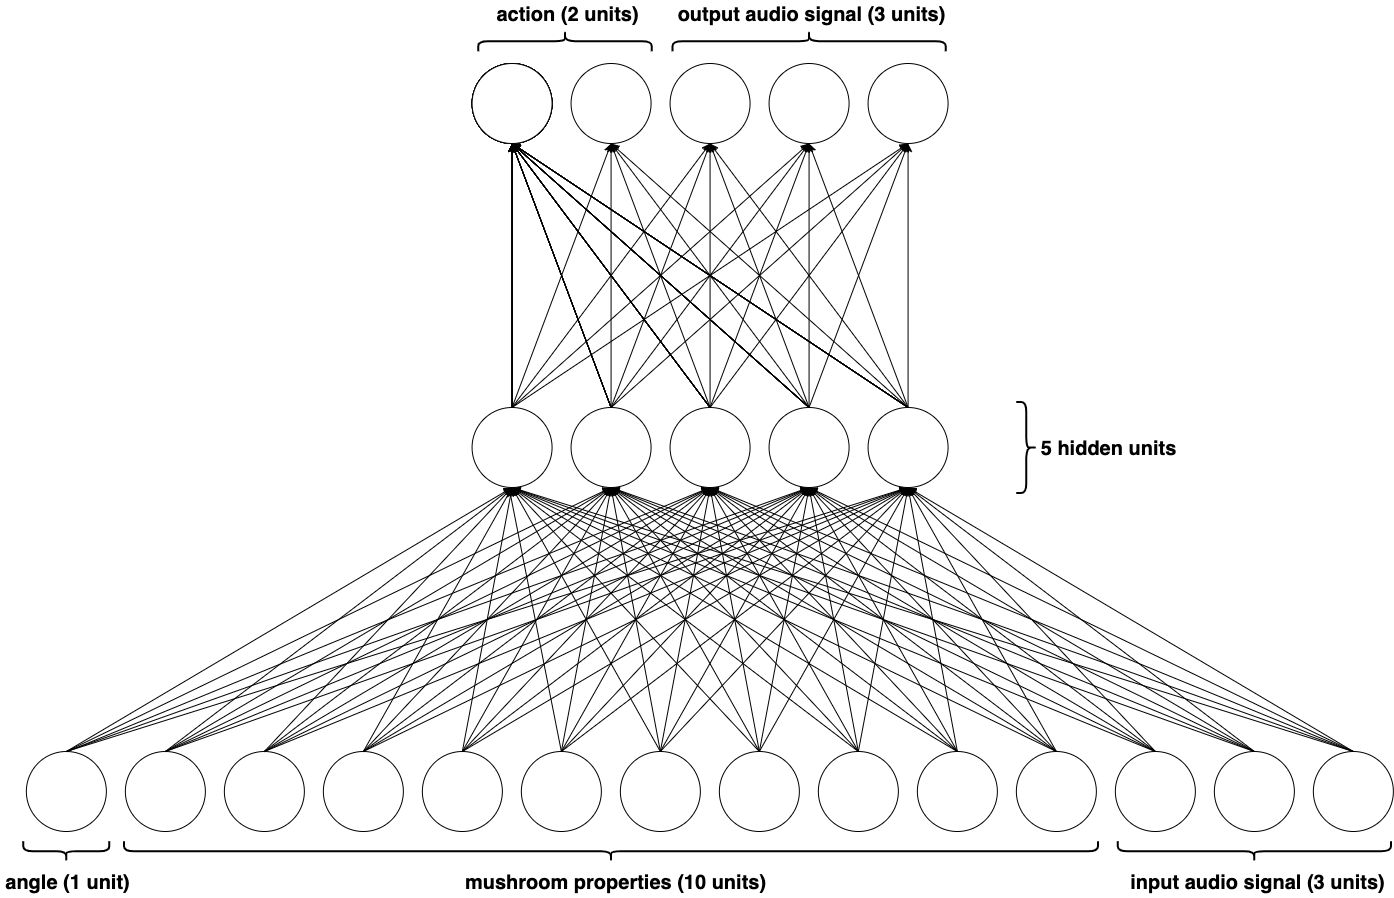
\includegraphics[width=.9\linewidth]{figs/fullneural}
  \caption{Fully-connected ANN to control entity behaviour}
  \label{fig:fullneural}
\end{figure}

\subsection{Reproduction}

\section{Simulation}\label{section:simulation}

\subsection{Single-Entity Simulation Run}

\subsection{Genetic Algorithm}

\subsection{Optimisations}\label{section:optimisations}

\subsection{Interactivity}

\subsection{Data Recording}

\section{Simulation Analysis}

\subsection{Fitness Graphs}

\subsection{Language Frequency Distributions}

\subsection{QI Score}

%%%%%%%%%%%%%%%%%%%%%%%%%%%%%%%%%%%%%%%%%%%%%%%%%%%%%%%%%%%%%%%%%%%%%%%
% Evaluation

\chapter{Evaluation}

\emph{Show graphs, run by run etc.}

\emph{Variance is interesting to discuss}

\emph{Could also be interesting to query what happens in an elbow in the graph - visual and a bit subjective. Three categories - those that don't take off, those that suddenly take off and those that gradually take off.}

\emph{Variance in each run, consequences of initialisation/activation, bigger questions about how reliable neural networks are, whether they're a good model for language evolution. }

%%%%%%%%%%%%%%%%%%%%%%%%%%%%%%%%%%%%%%%%%%%%%%%%%%%%%%%%%%%%%%%%%%%%%%%
% Conclusion

\chapter{Conclusion}

%%%%%%%%%%%%%%%%%%%%%%%%%%%%%%%%%%%%%%%%%%%%%%%%%%%%%%%%%%%%%%%%%%%%%
% the bibliography
\addcontentsline{toc}{chapter}{Bibliography}
\bibliography{refs}
\bibliographystyle{apalike}

%%%%%%%%%%%%%%%%%%%%%%%%%%%%%%%%%%%%%%%%%%%%%%%%%%%%%%%%%%%%%%%%%%%%%
% the appendices
\appendix

\chapter{Project Proposal}

\documentclass[12pt]{article}
\usepackage{a4wide}
\usepackage{datetime}
\usepackage{url}
\usepackage{hyperref}
\usepackage[svgnames]{xcolor}
\hypersetup{
  colorlinks,
  urlcolor=Blue}

\newcommand{\al}{$<$}
\newcommand{\ar}{$>$}
\newcommand{\sups}{\textsuperscript}
\newcommand{\belgianspacing}{\frenchspacing}

\parindent 0pt
\parskip 6pt

\begin{document}

\belgianspacing

\thispagestyle{empty}

%\rightline{\large\emph{Z\'ebulon Goriely}}
%\medskip
%\rightline{\large\emph{Queens'}}
%\medskip
%\rightline{\large\emph{zg258}}

%\vfil

\centerline{\large Computer Science Part II Project Proposal}
\vspace{0.2in}
\centerline{\Large\bf Simulating Language Learning and Evolution}
\vspace{0.2in}
\centerline{\large {\bf{Z\'ebulon Goriely --- Queens' --- zg258}}}
\vspace{0.2in}
\newdate{proposaldate}{18}{10}{2019}
\centerline{\large {\displaydate{proposaldate}}}
 
 \vspace{0.3in}
 
%\vfil

{\bf Project Originator:} Z\'ebulon Goriely

{\bf Project Supervisor:} {Prof. Paula Buttery and Dr. Andrew Caines}

{\bf Director of Studies:}  {Prof. Alastair Beresford}

{\bf Overseers:} {Prof. Pietro Lio’} and {Dr. Robert Mullins}

\section*{Introduction}

Language has evolved and therefore probably gave an evolutionary advantage to the individuals that exhibited it. As Angelo Cangelosi and Domenico Parisi described in a 1998 paper\footnote{\url{https://doi.org/10.1080/095400998116512}}, it is difficult to investigate the evolutionary origin of language and the selective pressures that may have originated language due to the limited evidence available. They propose using computer simulations of evolutionary scenarios to investigate this. In the paper referenced, they describe a simulated toy world where agents controlled by neural-networks interact with an environment of mushrooms that are edible and poisonous. This simulation and the ideas explored in the paper will be the basis for my project.

In the paper, Cangelosi and Parisi use small feed-forward neural networks to control the behaviour of each agent. The weights are initially random; a genetic algorithm is used to improve the fitness of the species over many generations. The agents are also given linguistic abilities; input and output nodes of the neural networks produce signals that allow for communication.

By creating three different populations (one without language, one with an externally imposed language and one with an evolved language) we can investigate the evolutionary advantage of language. Furthermore, it allows us to investigate a key question posed in the paper: \emph{``Since language requires the parallel evolution of linguistic production and linguistic comprehension, how can language evolve when it has a purely informative function and therefore it is advantageous to the receiver but not the producer?''}

For this project, I will re-implement the simulation described. I will then create analysis tools to investigate the findings of the paper to see if I observe the same results.

\section*{Starting Point}

I have a small amount of experience in programming simulations; for my A-Level project in 2016, I created a simulation of virus propogation between mosquito and human agents in the Unity game engine.

I do not have any experience programming neural networks, however, I am confident that I understand the backpropagation algorithm and basic neural network structure through the Artificial Intelligence course I took last year. In the papers I plan to reference, Cangelosi very clearly describes the structure of the neural networks he uses and I am confident that I will be able to follow his work.

Over the summer I read a book titled Simulating the Evolution of Language which gave me an overview of the techniques used in this field. Alongside the Formal Models of Language course that I took last year, I now have a sufficient base of understanding to begin this project.

\section*{Work to be Done}

The work for this project can be roughly divided into two stages; implementing the simulation and constructing the means of evaluating my implementation against the findings in the original paper. I will also regularly be creating tests to evaluate my simulation.

\subsection*{Implementing the Simulation}

\begin{enumerate}

\item Set up the simulation environment by creating the world grid and implementing the properties of poisonous and edible mushrooms. Create the simulation loop divided into regular `epochs'.

\item Create the agents for the simulation, giving them position and energy properties.

\item Implement feedforward neural networks to control the behaviour of the agents; input units to identify the location of the nearest mushroom, visual perception units to observe mushroom properties (only when close enough) and signal perception units for when language is implemented. The output units control the movement of the agent and production of signals. There will also be hidden units.

\item Implement the genetic algorithm that runs after all agents complete the simulation. The fittest agents are determined by the energy level (based on eating edible mushrooms and avoiding poisonous mushrooms). The fittest agents are then chosen for asexual reproduction, producing offspring that have genetic mutations in the form selecting a percentage of the weights to change by a random amount.

\item Create two different populations, one without language (where the signal perception units are always set to the same, constant value) and one with an externally imposed language (where the signal perception units are set to one of two signals depending on the type of the nearest mushroom).

\item Create a third population with an evolved language. Instead of externally imposed signals, in each simulation cycle one of the other agents is randomly selected as the `speaker' and its output is connected to the input signal perception units of the `listener'. 

\end{enumerate}

\subsection*{Analysis}

\begin{enumerate}

\item Plot the average fitness over the number of generations to compare between the three populations.

\item Produce some behavioural tests to investigate the behaviour of random individual organisms at specific generations.

\item Plot the frequency distribution of the different signals produced by the individuals with the evolved language using a `naming task'.

\item Calculate the Quality Index (QI) of the language produced by the population without language and the population with an evolved language to investigate the genetic advantage of producing productive signals. The QI evaluates the efficiency of a language based off of three criteria; (1) functionally distinct categories are labeled with distinct signals, (2) a single signal tends to be used to label all the instances within a category and (3) all the individuals in the population tend to use the same signal to label the same category.

\item Investigate the correlation between QI of the language and the fitness of the species to determine if change in the language or in the categorisation skill of the agents affects the other ability.

\end{enumerate}

\subsection*{Testing}

To evaluate my project and ensure that my simulation implementation is functional, I will create an ensemble of unit tests for each of the tasks above. These will be created in parallel as I develop each part of the implementation. For the simulation, this will involve small examples or scenarios to show that each part of the simulation is fully functional.

\section*{Success Criterion}

The project will be deemed a success if I can implement the simulation as described in the tasks above (evaluated by my unit tests) and if I can implement the analysis tools to compare the findings of my implementation to the findings of the original paper.

\section*{Timetable and Milestones}

I've broken down this timetable into two and three week intervals. At the end of December, I will be writing my Progress Report and simultaneously making adjustments to the timetable as needed.

\subsection*{25\sups{th} October -- 10\sups{th} November}

\emph{Middle of Michaelmas Term. Includes first deadline for NLP coursework.}


{\bf Task:} Create a high-level design of the system. Set up the project files with a version-control system. Experiment with creating small simulations in python and do suitable research into Neural Network libraries.

{\bf Milestones:} Have a git repository with project files. Have a design plan with specific details of the simulation confirmed.

\subsection*{11\sups{th} November -- 24\sups{th} November}

\emph{Middle of Michaelmas Term.}


{\bf Task:} Complete implementation tasks 1 and 2 as described above. Experiment with adding Neural Networks to control the behaviour of the agents.

{\bf Milestones:} Have a working simulation environment with poisonous and edible mushrooms. Have agents with positions and energy values but no functional neural networks yet.

\subsection*{25\sups{th} November -- 8\sups{th} December}

\emph{End of Michaelmas Term. Includes second and third deadline for NLP coursework.}


{\bf Task:} Complete implementation tasks (3). Start working on implementation task (4).

{\bf Milestones:} Have the agents successfully controlled by neural networks. Be able to run an entire lifespan of one agent within the simulated world. Have the beginnings of a 

\subsection*{9\sups{th} December -- 22\sups{nd} December}

\emph{Christmas holiday. Will likely be in Cambridge to help with Queens' interviews.}

{\bf Task:} Complete implementation tasks (4), (5) and (6). Also aim to complete analysis tasks (1) and (3).

{\bf Milestones:} Have a fully functional simulation that allows for running a thousand generations of a population of agents. Have three different populations to compare; one without language, one with an externally imposed language and one with an evolved language. Have a tool to graph the average fitness of each population over the number of generations and another tool to view the probability distribution of the signals chosen for the evolved language over the number of generations.

\subsection*{23\sups{rd} December -- 12\sups{th} January}

\emph{Christmas holiday. Will take a break to revise Michaelmas courses and to spend time with family.}

{\bf Task:} Complete analysis task (2). Write the Preparation chapter of the Dissertation. Review the timetable for the remainder of the project and adjust in light of experience so far. If ahead of schedule, plan time for extensions. Start to plan tests cases.

{\bf Milestones:} An outline of the dissertation document with a completed Preparation section.

\subsection*{13\sups{th} January -- 2\sups{nd} February}

\emph{Start of Lent term. Will have regular labs for Mobile Robot Systems.}

{\bf Progress Report Deadline:} 31\sups{st} January

{\bf Task:} Write the Progress Report. Start to fill out the Implementation chapter of the Dissertation. Complete analysis tasks (4) and (5).

{\bf Milestones:} Progress report submitted and entired project reviewed both personally and with overseers. Have tools to plot the Quality Index of the evolved language against the fitness of the population. At this point, all the tasks in the {\bf Work to Do} section will have been completed, satisfying the {\bf Success Criteria}.

\subsection*{3\sups{rd} February -- 23\sups{rd} February}

\emph{Middle of Lent term. Both deadlines for the Mobile Robot Systems assignments.}

{\bf Task:} Begin analysis of the simulation. Begin to work on extensions to the project, keeping in mind time needed to write the Dissertation.

{\bf Milestones:} Have the start of a test suite with a series of diagrams to use to evaluate my implementation.

\subsection*{24\sups{th} February -- 15\sups{th} March}

\emph{End of Lent term. Deadline for the Mobile Robot Systems mini-project report.}

{\bf Task:} Complete testing. Evaluate the outcomes of the tests against the findings in the original paper. At this point, the second half of the {\bf Success Criteria} will have been achieved. If needed, revise the implementation to be clean, documented and consise. Work on other extensions.

{\bf Milestones:} Examples and test cases run with results collected. Code should perform a variety of interesting tasks and should be in a state that in the worst case it would satisfy the examiners with at most cosmetic adjustment

\subsection*{16\sups{th} March -- 5\sups{th} April}

\emph{Start of Easter holiday. Might stay in Cambridge for part of it to work. Will balance revision and work on the project.}

{\bf Task:} Complete work on any extensions. Draft the Evaluations and Conclusions chapters of the Dissertation.

{\bf Milestones:} Extensions almost complete. Skeleton of entire Dissertation in place.

\subsection*{6\sups{th} April -- 19\sups{th} April}

\emph{End of Easter holiday. Might get back to Cambridge early to work. Will balance revision and work on the project.}

{\bf Task:} Complete the Implementation and Introduction chapters of the Dissertation. Send the full draft to Director of Studies and Supervisors by 21st of April.

{\bf Milestones:} Dissertation essentially complete, with large sections of it proof-read by Supervisors and possibly friends and/or Director of Studies.

\subsection*{20\sups{th} April -- 8\sups{th} May}

\emph{Start of Easter Term. Will be balancing revision, lectures and final work on the project.}

{\bf Final Deadline:} 8\sups{th} May

{\bf Task:} Finish Dissertation, preparing diagrams for insertion. Review the whole project, checking the Dissertation and spending the final few days on whatever is in greatest need of attention. Aim to submit the dissertation at least a week before the deadline.

{\bf Milestone:} Submission of Dissertation

\section*{Possible Extensions}

\subsection*{Graphic Visualisation}

As a side extension, I could implement a visual interface to watch the life of one agent within the simulation. This would involve rendering a simple 2D world with textures for the agents and mushrooms. This could be expanded further by adding a User Interface for setting up the simulation and having windows showing the progress as it occurs live.

\subsection*{Symbolic Theft vs. Sensorimotor Toil}

In a 2000 paper\footnote{\url{http://cogprints.org/2036/}}, Cangelosi and Harnad use a similar same toy world of mushrooms and foragers to place two ways of acquiring categories in direct competition with each other. They compare ``sensorimotor toil'' (where categories are acquired through real-time, feedback-correct, trial and error experience) to ``symbolic theft'' (where new categories are acquired by hearsay from boolean combinations of symbols \emph{describing} them). They find that the origins of natural language could be explained by the apparent infinitely superiority of a hybrid symbolic/sensorimotor combination compared to purely sensorimotor precursors. 

As an extension, I could expand my simulation to investigate the findings of this paper. This involves implementing a more complicated neural network, adding supervised learning through back-propagation, implementing more sophisticated mushroom features and expanding the simulation to host multiple populations at once.

\subsection*{Investigating the Evolution of Syntax}

In a 1999 paper\footnote{\url{https://link.springer.com/chapter/10.1007/3-540-48304-7_86}}, Cangelosi expands the toy mushroom world simulation further to investigate how languages that use combinations of words (such as the ``verb-object'' rule) can emerge by auto-organisation and cultural transmission. Mushrooms are either edible or poisonous but also have one of three colours - the edible mushrooms of a particular colour correspond to a particular action in response.

In this extended simulation, after the first 300 generations parents and children co-exist within the simulated world. Parents teach the evolved language to their children. Children undergo a Listening Task (where parents describe the closest mushroom) and a Naming Task (where the mushroom name is used for supervised learning through backpropagation).

This is a substantial increase in complexity but allows would allow me to investigate the evolution of a more complex language.

 \section*{Resources Declaration}

For this project, I plan to use my computer, (2.8 GHz CPU, 16 GB RAM, 750GB Flash Storage,
macOS Mojave). The code will be regularly pushed to a GitHub repository to be able to recover from failure or loss on my local machine. I will also create weekly backups on an external hard-drive to provide another source of recovery. Should my machine fail, I will be able to continue working on an MCS machine. I accept full responsibility for this machine and I have made contingency plans to protect myself against hardware and/or software failure. 

I will also need to use the high powered computer when running large simulations to save processing time.

 \end{document}




\end{document}
